% Compiler: LaTeX => PDF

\documentclass[xcolor=dvipsnames]{beamer}

\mode<presentation>
{
	\usetheme{BerlinHUB}
	%\setbeamercovered{transparent}
}

\usepackage[ngerman]{babel}
\usepackage[utf8]{inputenc}

\usepackage{helvet}
\usepackage[T1]{fontenc}

%\usepackage{multimedia}
%\usepackage{graphicx}
%\usepackage[nolist]{acronym}

%\usepackage{stackengine}
%\usepackage{array}

%\usepackage{enumitem}

\def\frametitlesec{\frametitle{\arabic{section}.\hspace{0.5ex}\insertsection}}
\def\framesubtitles#1{\framesubtitle{\hspace{3.5ex}#1}}

%\setitemize{label=\usebeamerfont*{itemize item}%
%  \usebeamercolor[fg]{itemize item}
%  \usebeamertemplate{itemize item}}

\title[Streifenlichtprojektion]
{Streifenlichtprojektion und optische Analyse zur Oberflächeninspektion}

\author[D. Wagner, J. Spangenberg, L. Kramer]
{
	Dennis~Wagner
	\and
	Johannes~Spangenberg
	\and
	Leroy~Kramer
}

\institute[]
{
	Humboldt-Universität zu Berlin\\  
	Institut für Informatik\\
	Lehrstuhl Signalverarbeitung und Mustererkennung\\
	\vspace{1em}
	Semesterprojekt Signalverarbeitung\\
	bei Prof. Dr. Meffert
}

\date{12.02.2014}
\subject{Informatik}

% add logo of university
\pgfdeclareimage[height=0.75cm]{university-logo}{husiegel_bw_klein}
\logo{\pgfuseimage{university-logo}}

\setbeamercolor*{block title}{fg=white, bg=HUblue}


\begin{document}
\begin{frame}
	\frametitle{\mbox{}}
	\titlepage
\end{frame}

\begin{frame}
	\frametitle{Gliederung}
	\tableofcontents
\end{frame} 

% ---------------------------------------------------------------------------- %

\section{Motivation}
\begin{frame}
	\frametitlesec

	\textbf{Wie gelangt man an die Ausmaße eines Objektes?}
	\vfill
	\begin{itemize}
		\item Manuell vermessen zu aufwendig
		\item Stereo-Vision?\\
		Benötigt eindeutig wiedererkennbare Muster!
		\item Structure from Motion? s. Stereo-Vision!
		\item Time of Flight?\\
		Geringe Auflösung!\\
		Für manche Anwendungsgebiete zu ungenau!
	\end{itemize}
	\vfill
	\textbf{Unsere Methode: Streifenlichtprojektion}
	\vfill

\end{frame}


\begin{frame}
	\frametitlesec
	\framesubtitles{Anwendungsgebiete}

	\begin{itemize}
		\item Computer Grafik
		\item Robotik
		\item Archäologie
		\item Geographie
		\item Reverse Engineering
		\item Computerunterstütze Qualitätskontrolle
		\item \dots
	\end{itemize}

\end{frame}


\begin{frame}
	\frametitlesec
	\framesubtitles{Vor- und Nachteile}

	\textbf{Vorteile}
	\vfill
	\begin{itemize}
		\item Relativ günstig
		\item Messung ohne Kontakt zum Objekt
		\item Hohe Genauigkeit möglich
		\item Keine Korrespondenzsuche
	\end{itemize}
	\vfill
	\textbf{Nachteile}
	\vfill
	\begin{itemize}
		\item Langsam (im Vergleich zu \textit{Time of Flight})
		\item Abschattung des Lasers
	\end{itemize}
	\vfill

\end{frame}

% ---------------------------------------------------------------------------- %

\section{Umsetzung}
\begin{frame}
	\frametitlesec

	\begin{figure}
		\centering
		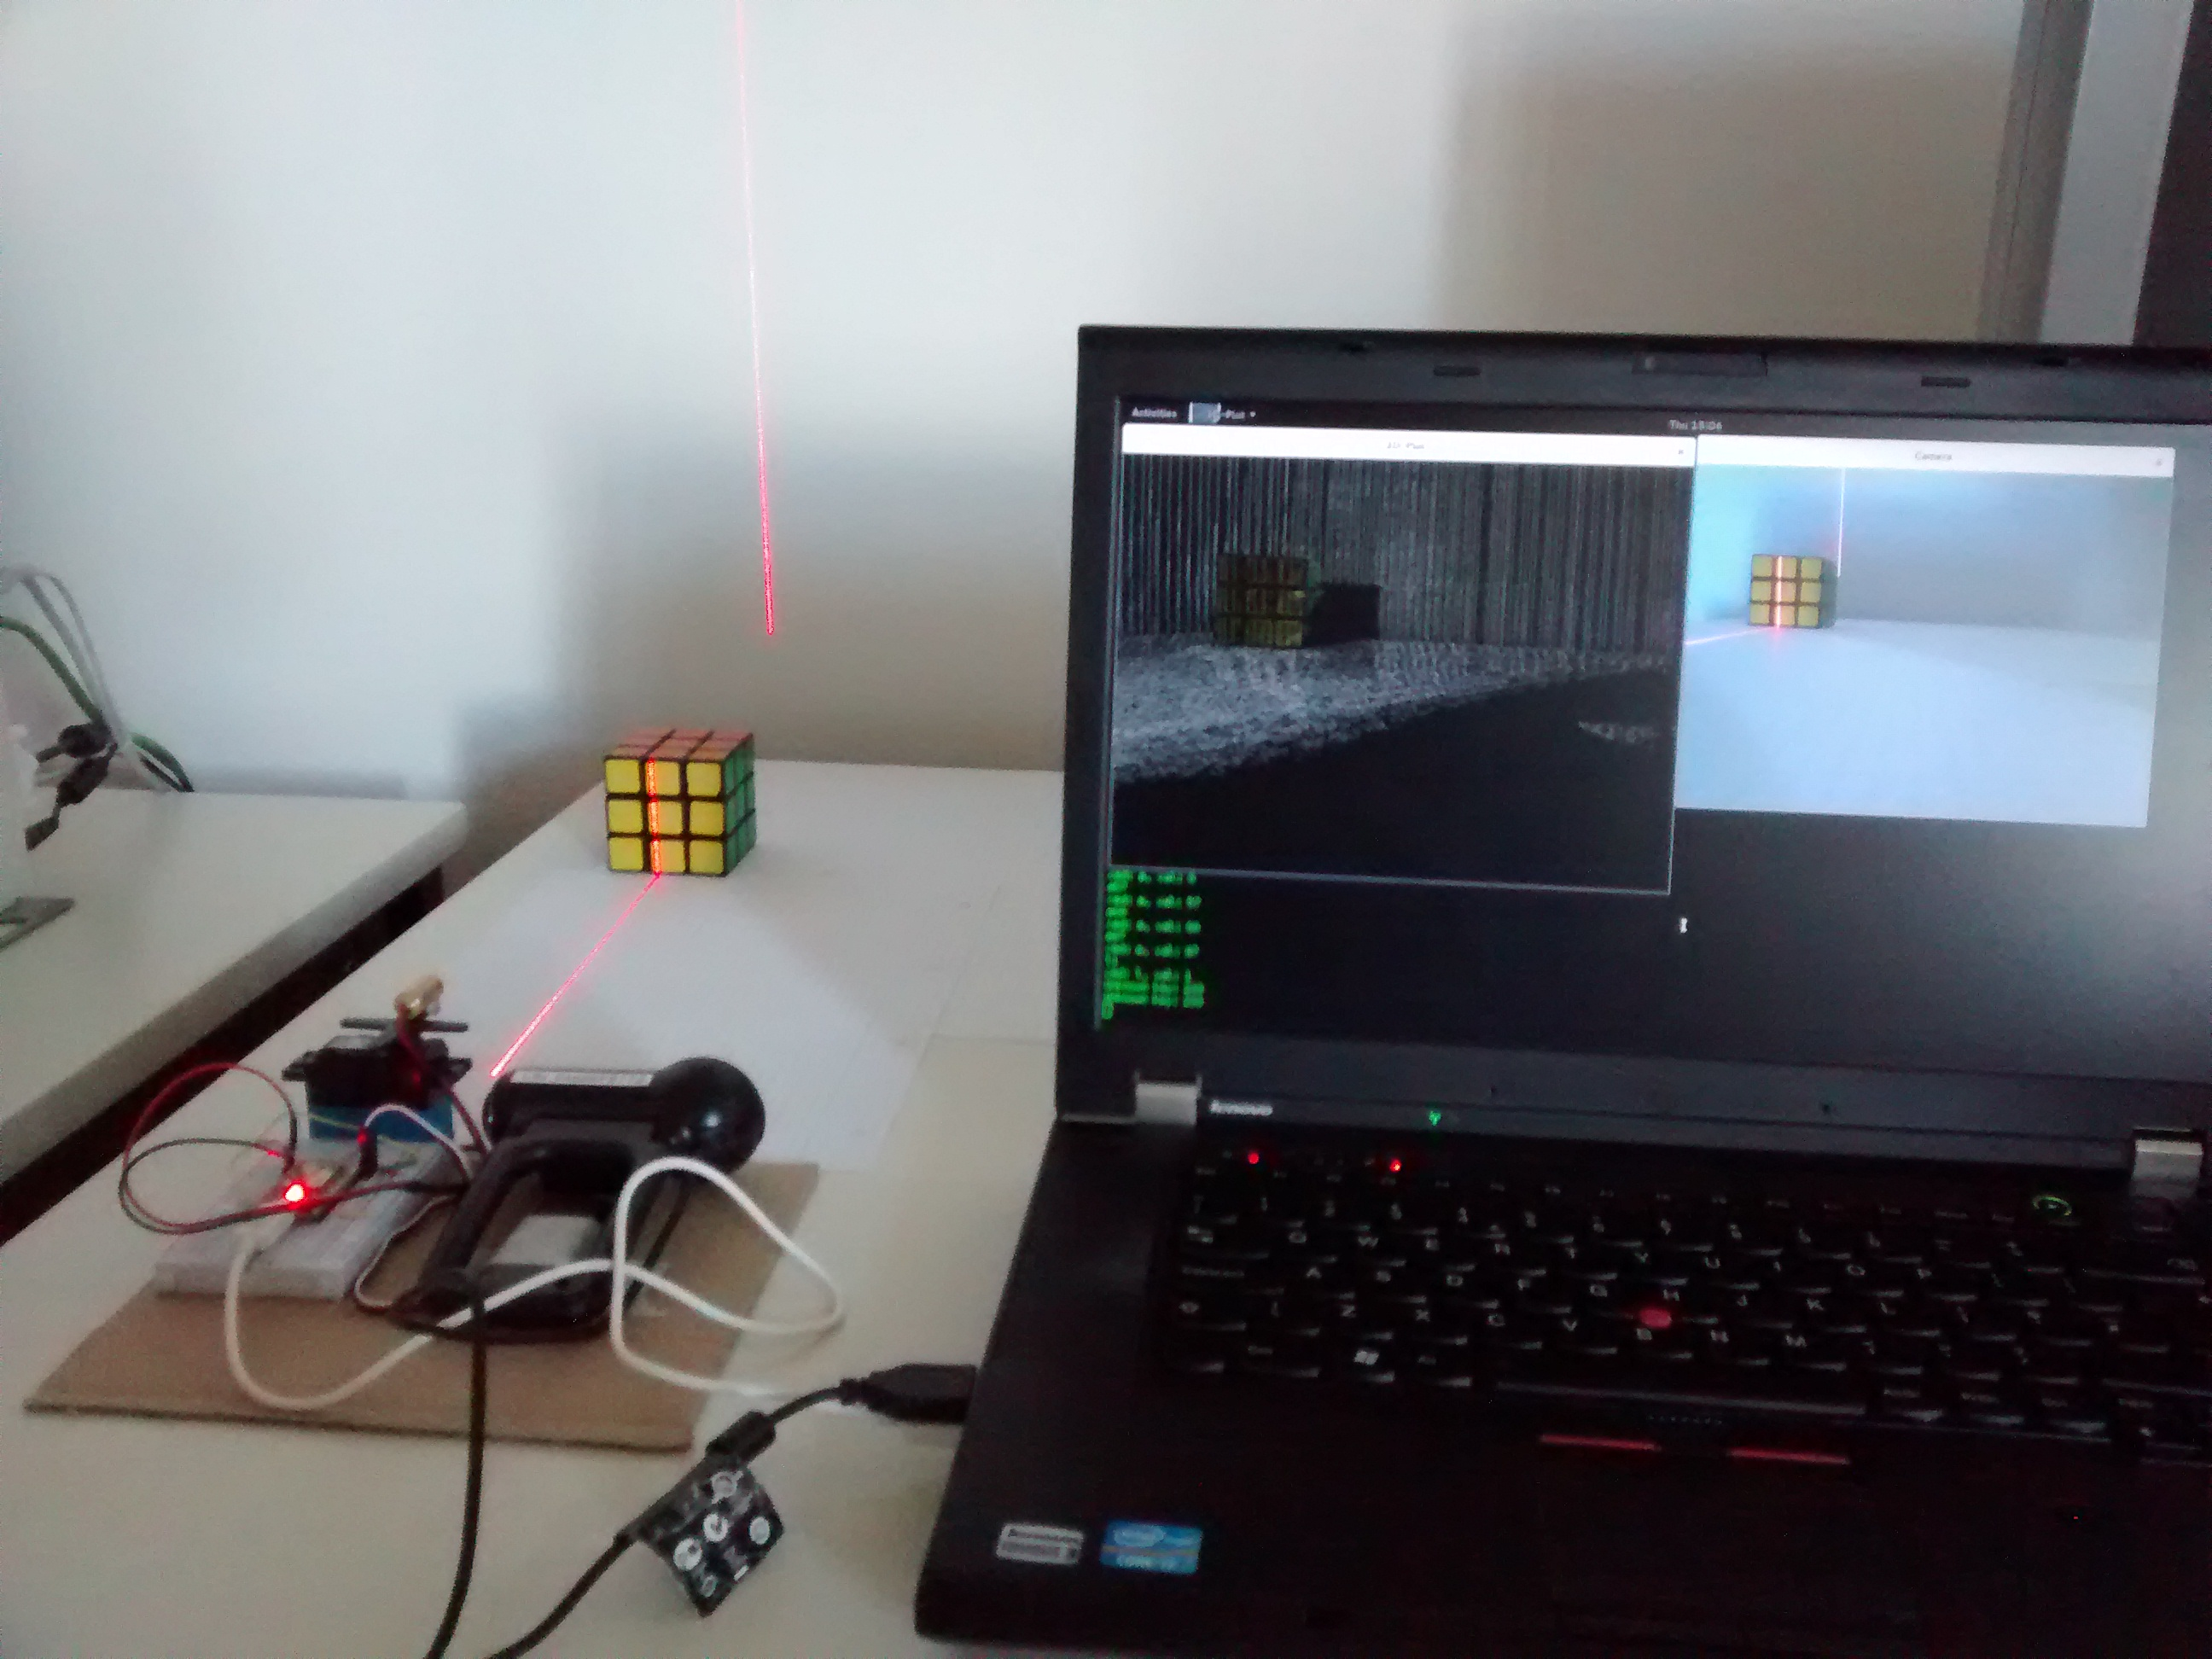
\includegraphics[width=0.8\linewidth]{includes/setup}
		\caption{Unser Setup im Betrieb}
		\label{fig:setup}
	\end{figure}

\end{frame}


%\subsection{Hardware}
\begin{frame}
	\frametitlesec
	\framesubtitles{Hardware}

	\begin{figure}
		\centering
		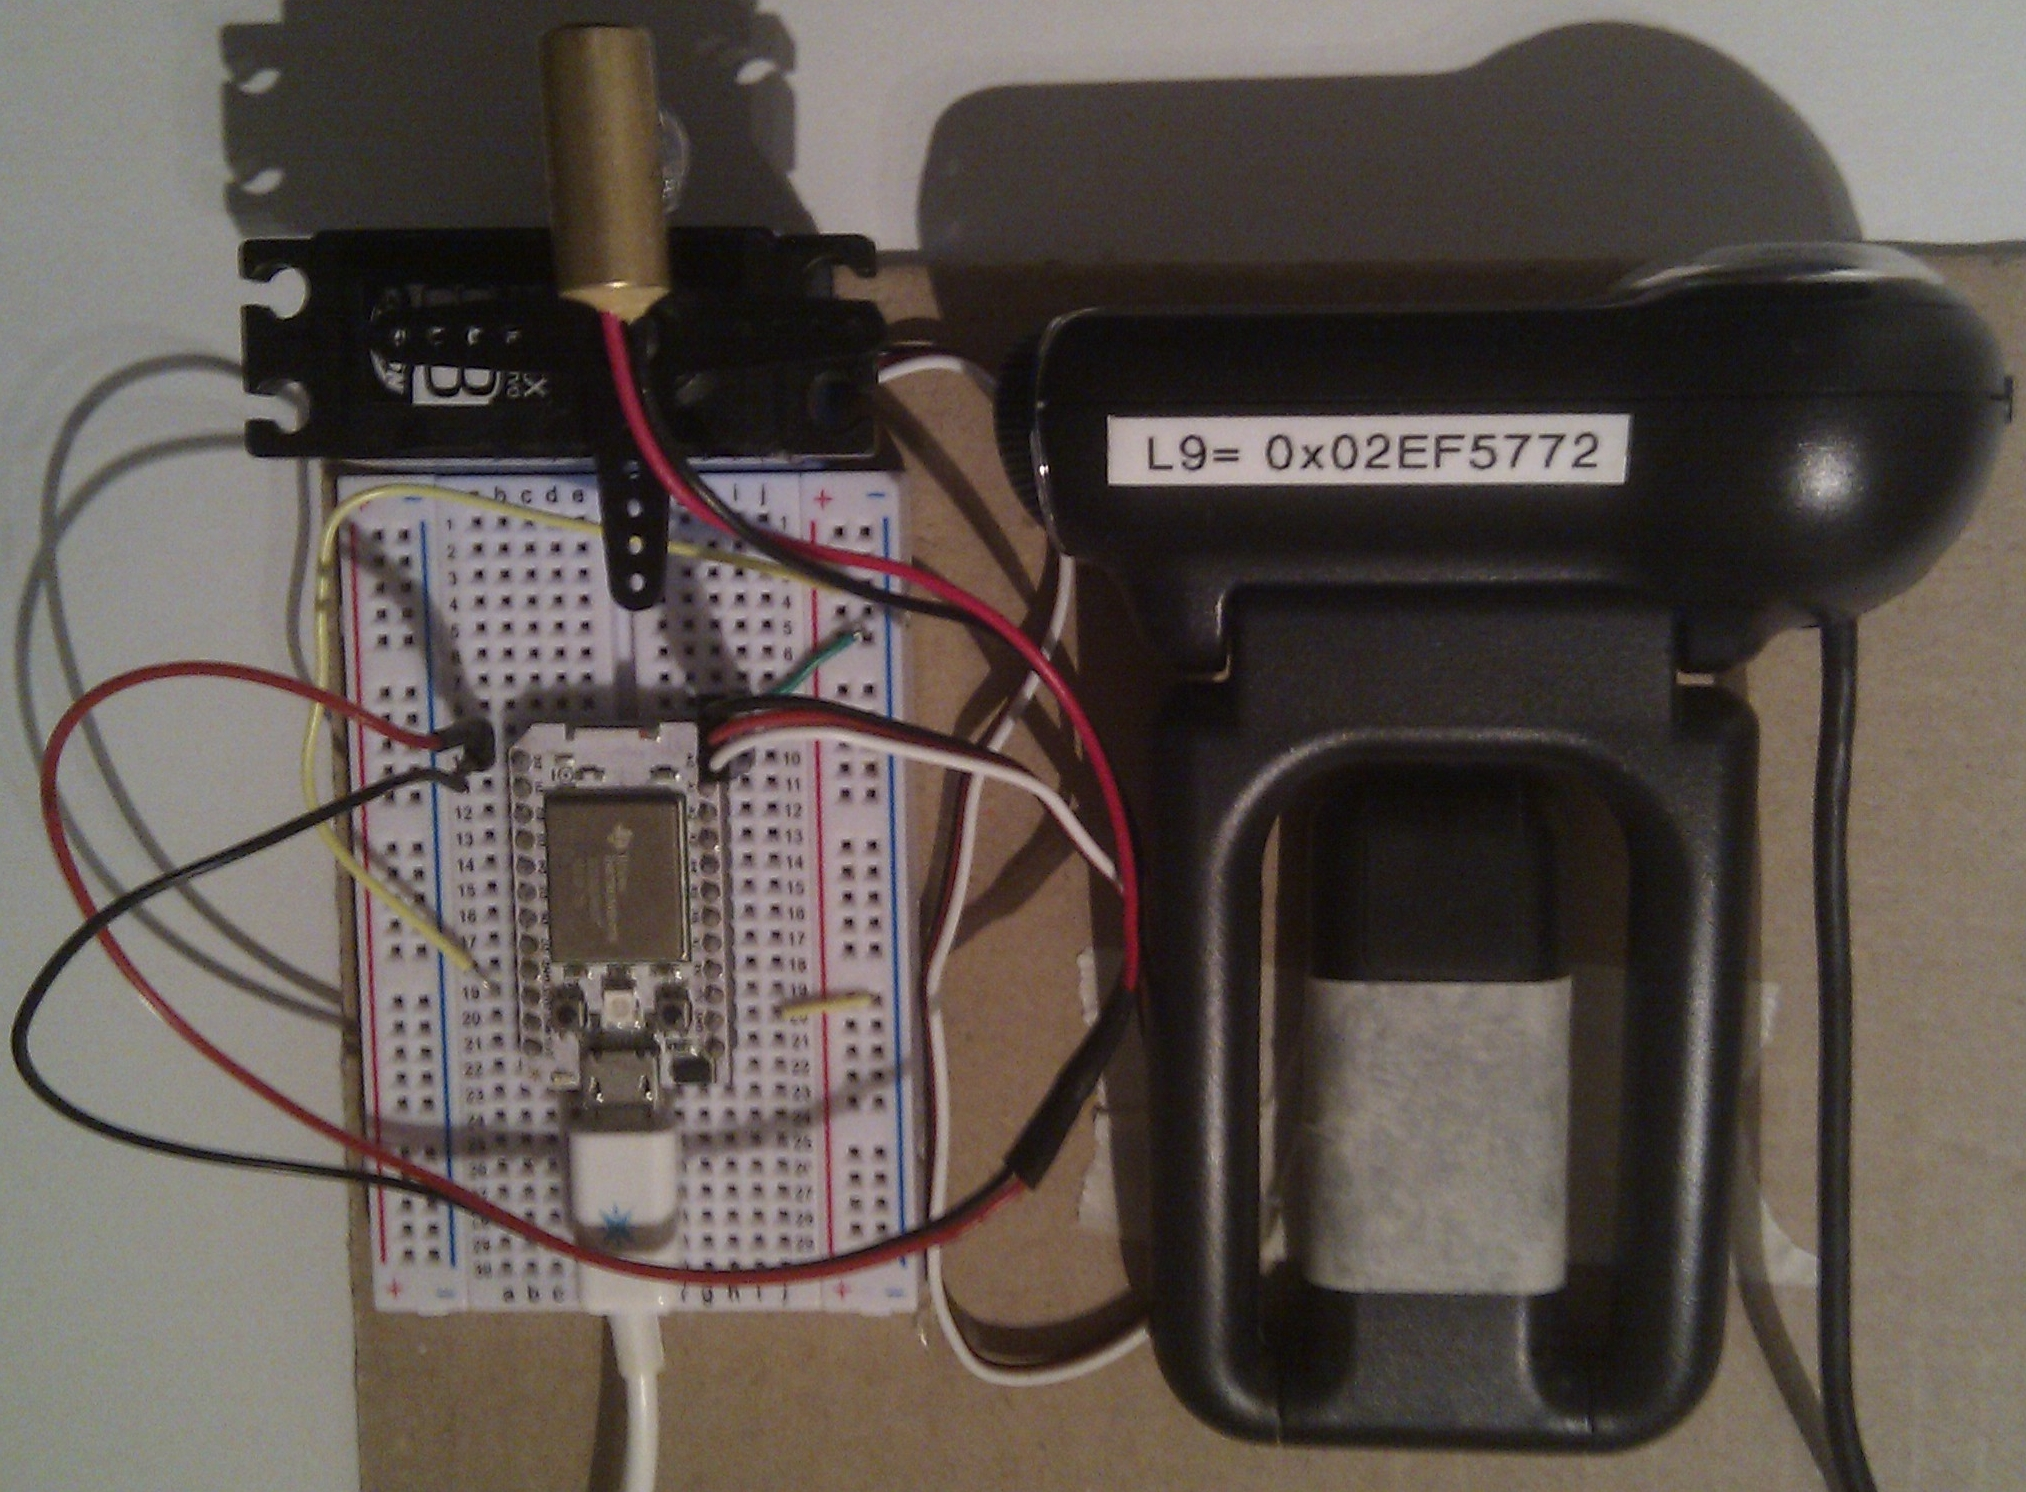
\includegraphics[width=0.8\linewidth]{includes/hardware.jpg}
		\caption{Unsere Hardware}
		\label{fig:hardware}
	\end{figure}

\end{frame}


%\subsection{Ablauf}
\begin{frame}
	\frametitlesec
	\framesubtitles{Ablauf}

	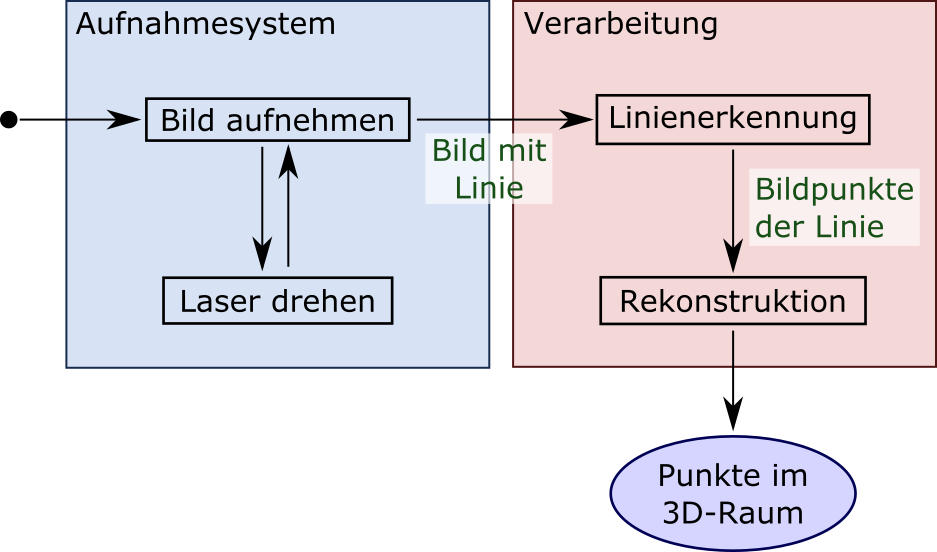
\includegraphics[width=\linewidth]{includes/blockbild.png}

\end{frame}


%\subsection{Linienerkennung}
\begin{frame}
	\frametitlesec
	\framesubtitles{Linienerkennung}

	\textbf{Variante 1}\\
	Einfache Linienerkennung durch Differenzbildung:
	\vfill
	\begin{columns}
		\visible<1-4>{\column{.32\linewidth}{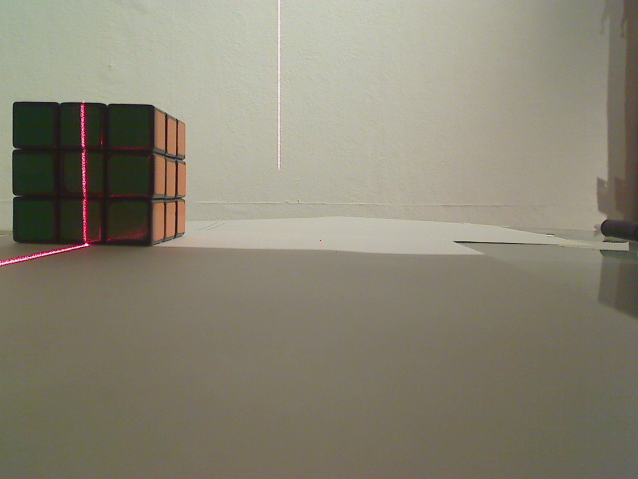
\includegraphics[width=\linewidth]{includes/line_line}}}
		\visible<2-4>{\column{.02\linewidth}{$-$}}
		\visible<2-4>{\column{.32\linewidth}{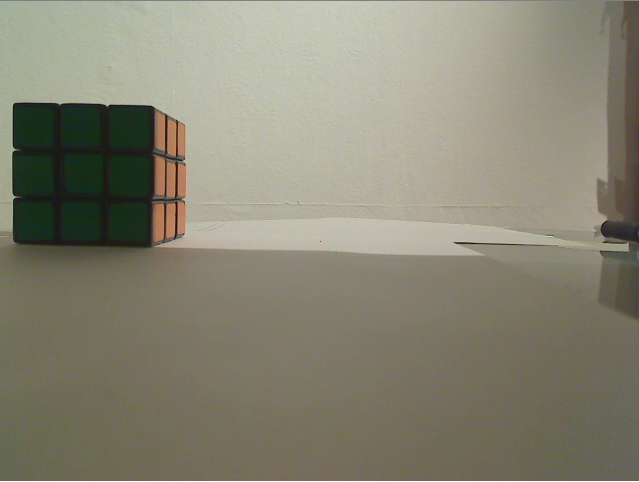
\includegraphics[width=\linewidth]{includes/line_ref}}}
		\visible<3-4>{\column{.02\linewidth}{$=$}}
		\visible<3-4>{\column{.32\linewidth}{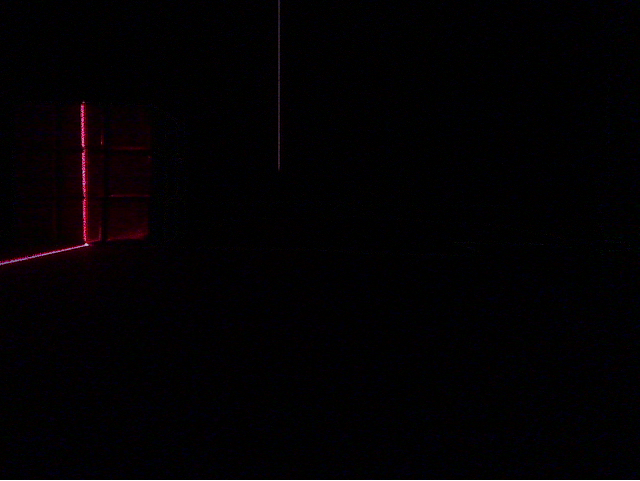
\includegraphics[width=\linewidth]{includes/line_diff}}}
	\end{columns}
	\vfill
	\begin{columns}
%		\column{.02\linewidth}{$\Rightarrow$}
		\visible<4>{\column{.41\linewidth}{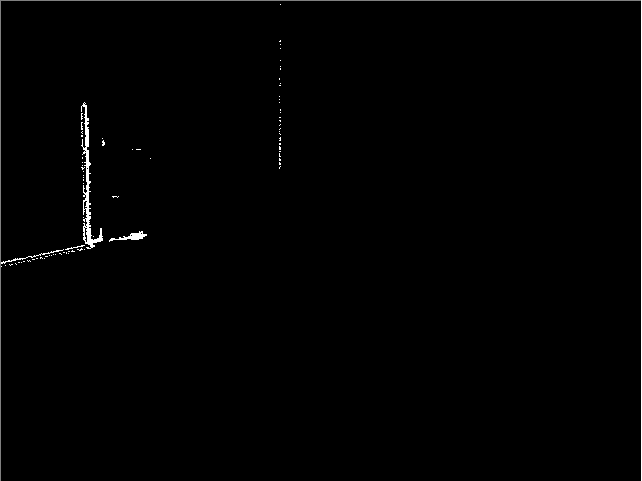
\includegraphics[width=\linewidth]{includes/line_diff_filtered}}}
	\end{columns}

\end{frame}


\begin{frame}
	\frametitlesec
	\framesubtitles{Linienerkennung}

	\textbf{Variante 2}\\
	Linienerkennung durch kanalweise Mittelwertbildung und logische Verknüpfung:
	\vfill
	\begin{columns}
		\visible<1-2>{\column{.45\linewidth}{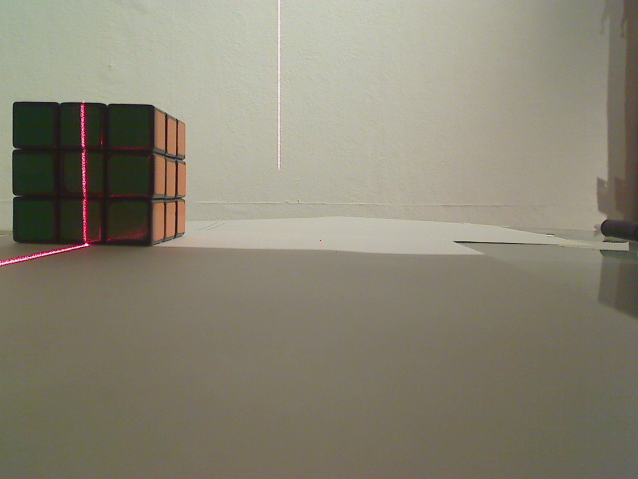
\includegraphics[width=\linewidth]{includes/line_line}}}
		\visible<2>{\column{.05\linewidth}{$\Rightarrow$}}
		\visible<2>{\column{.45\linewidth}{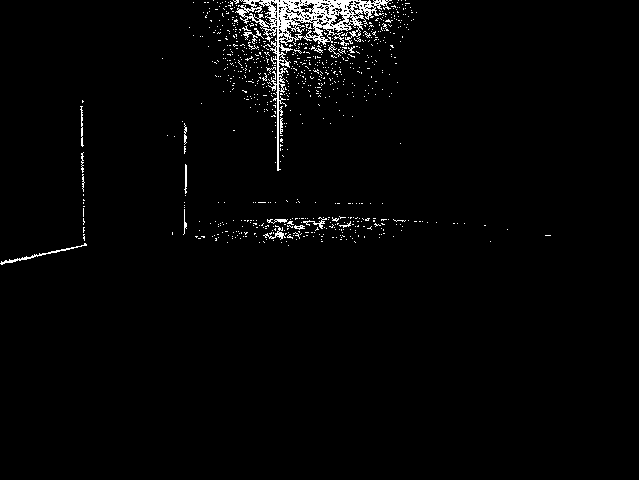
\includegraphics[width=\linewidth]{includes/line_free}}}
	\end{columns}

\end{frame}


%\subsection{Rekonstruktion}
\begin{frame}
	\frametitlesec
	\framesubtitles{Rekonstruktion}

	\begin{columns}
		\small
		\begin{column}{.61\linewidth}
			\begin{itemize}
				\item \textbf{Eingabe:} Normalisierte Bildkoordinaten $(u,v)$ eines Punktes der Laserlinie
				\item \textbf{Schritt 1:} Bestimme $\alpha$, $\beta$, $c$ und $f$
				\item \textbf{Schritt 2:} Berechne $h$:
				\[h = \frac{c \cdot \sin(\alpha) \cdot \sin(\beta)}{\sin(180^\circ - \beta - \alpha)}\]
				\item \textbf{Schritt 3:} Bestimme Koordinaten innerhalb der Szene:
				\[\begin{pmatrix}x\\y\\z\end{pmatrix} = \frac{h}{f} \cdot
				\begin{pmatrix}u\\v\\-f\end{pmatrix}\]
			\end{itemize}
		\end{column}
		\begin{column}{.39\linewidth}
			\hfill\fbox{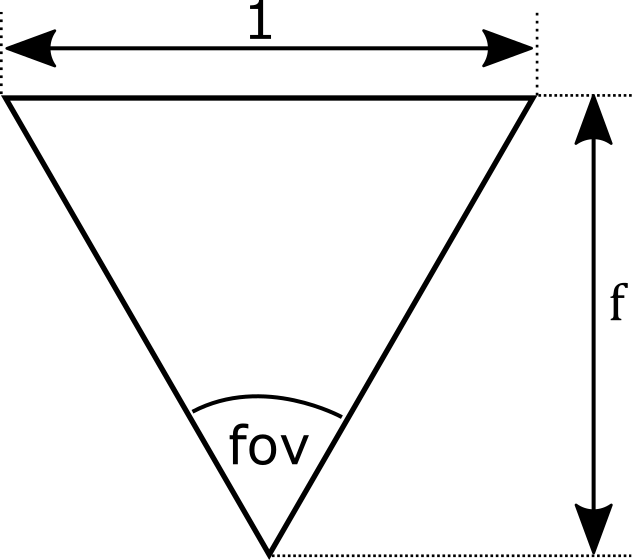
\includegraphics[width=0.9\linewidth]{includes/reconstruction_2}}
			\vfill\vspace{3ex}\vfill
			\hfill\fbox{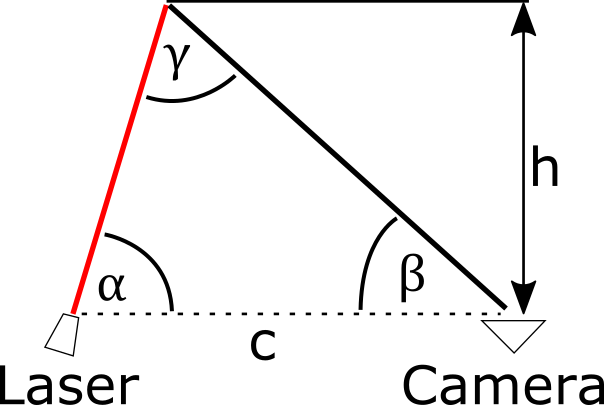
\includegraphics[width=0.9\linewidth]{includes/reconstruction_1}}
		\end{column}
	\end{columns}

\end{frame}


%\subsection{Beispiel}
\begin{frame}
	\frametitlesec
	\framesubtitles{Beispiel}

	\begin{overlayarea}{\textwidth}{\textheight}
		\only<1>{
			\begin{figure}
				\centering
				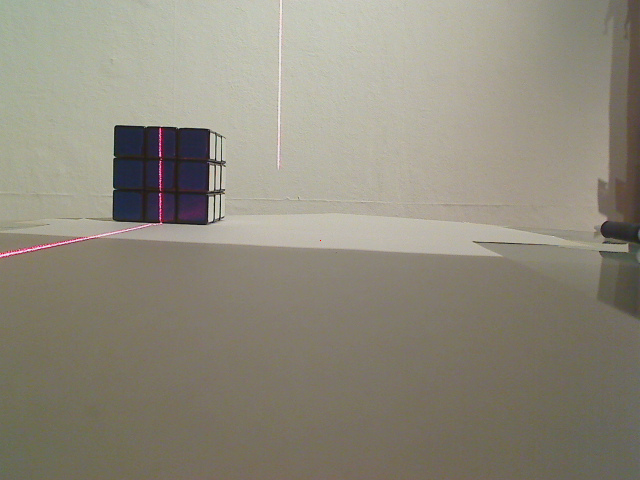
\includegraphics[width=0.8\linewidth]{includes/cap.png}
				\caption{Ausgangsbild}
				\label{fig:example1}
			\end{figure}
		}
		\only<2>{
			\begin{figure}
				\centering
				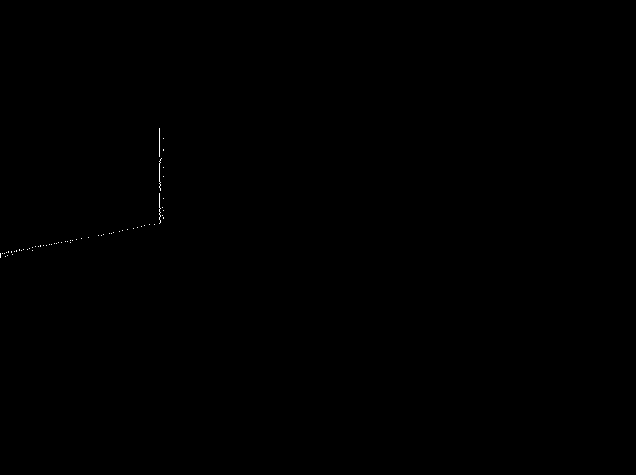
\includegraphics[width=0.8\linewidth]{includes/line.png}
				\caption{Erkannte Linie aus dem Ausgangsbild}
				\label{fig:example2}
			\end{figure}
		}
		\only<3>{
			\begin{figure}
				\centering
				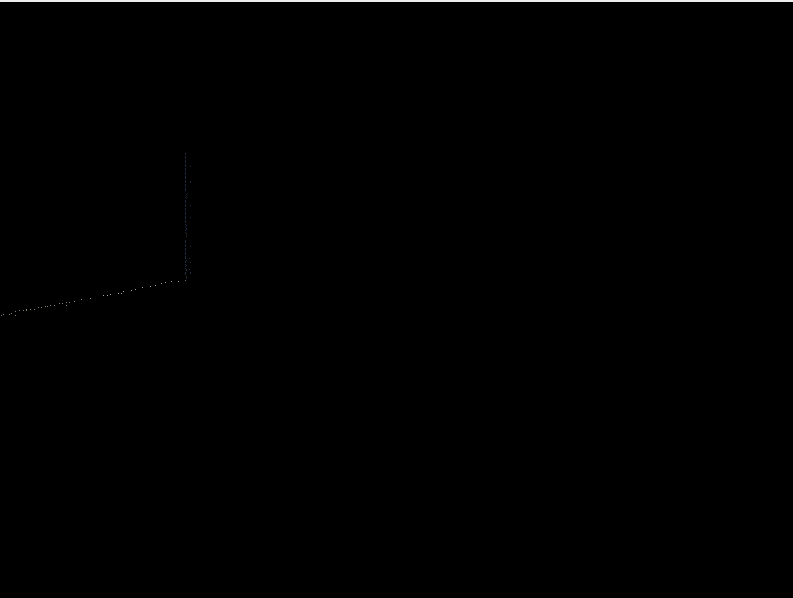
\includegraphics[width=0.8\linewidth]{includes/3d.png}
				\caption{Rekonstruierte Punkte aus der Perspektive der Kamera}
				\label{fig:example3}
			\end{figure}
		}
		\only<4>{
			\begin{figure}
				\centering
				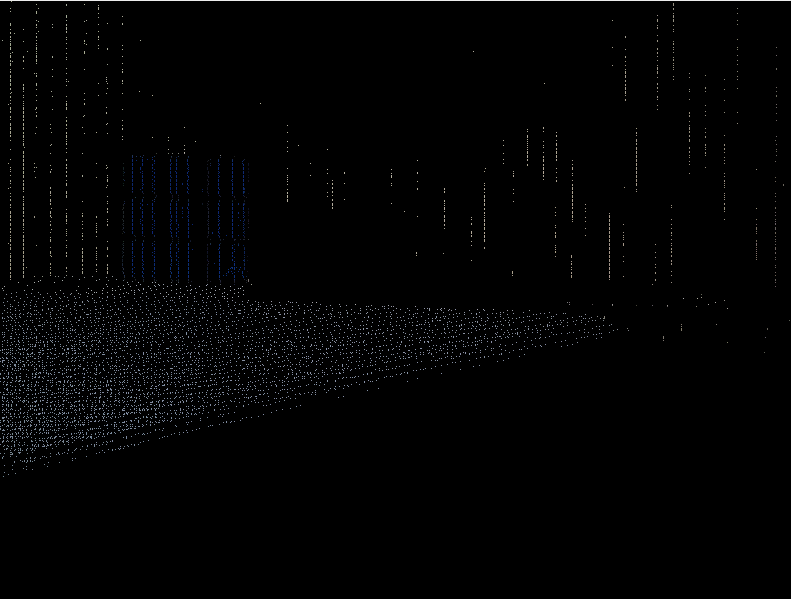
\includegraphics[width=0.8\linewidth]{includes/3d_2.png}
				\caption{Rekonstruierte Punkte der Szene (1)}
				\label{fig:example4}
			\end{figure}
		}
		\only<5>{
			\begin{figure}
				\centering
				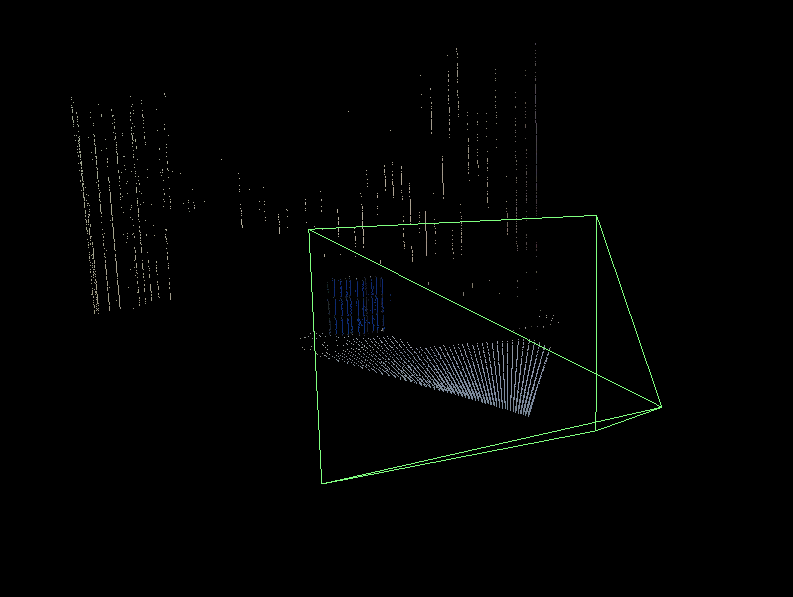
\includegraphics[width=0.8\linewidth]{includes/3d_3.png}
				\caption{Rekonstruierte Punkte der Szene (2)}
				\label{fig:example5}
			\end{figure}
		}
		\only<6>{
			\begin{figure}
				\centering
				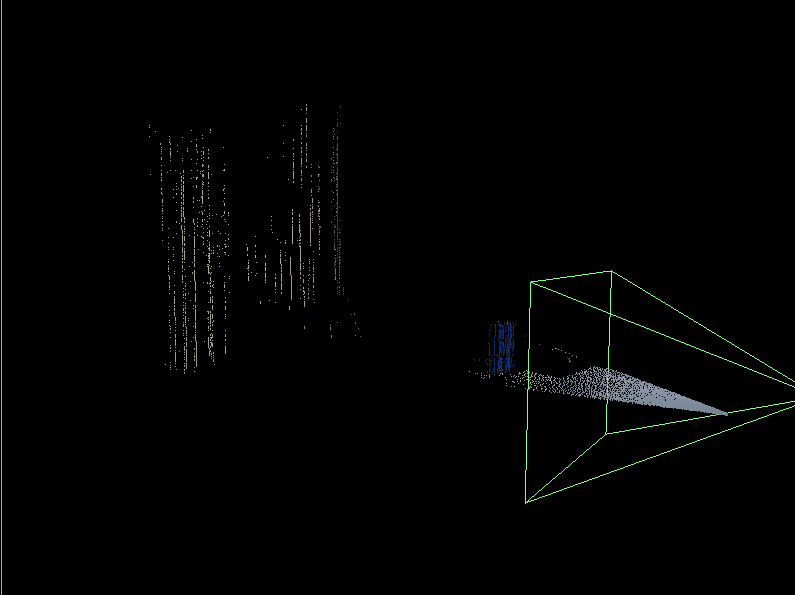
\includegraphics[width=0.8\linewidth]{includes/3d_4.png}
				\caption{Rekonstruierte Punkte der Szene (3)}
				\label{fig:example6}
			\end{figure}
		}
	\end{overlayarea}

\end{frame}

% ---------------------------------------------------------------------------- %

\section{Probleme}
%\subsection{Organisatorisches}
\begin{frame}
	\frametitlesec

	\begin{itemize}
		\item Viel Zeit bei der Planung verloren
		\begin{itemize}
			\item Fehlende Erfahrung bei der Strukturierung solcher Anwendungen
			\item Uneinigkeit bei Schwerpunkten und Verfahren
		\end{itemize}
		\item Aufbau der Hardware
		\begin{itemize}
			\item Montage von Laser auf Servo
			\item Montage der Kamera
		\end{itemize}
		\item Ursache für Ungenauigkeiten
		\begin{itemize}
			\item Kleine Fehler bei der Montage können u.U. zu großen Fehlern führen
			\item Schwer die Winkel und Entfernungen zwischen Kamera, Servo und Laser genau zu messen 
		\end{itemize}
		\item Liniernerkennung
		\begin{itemize}
			\item Hintergrundfarbe
			\item Beleuchtung
		\end{itemize}
	\end{itemize}

\end{frame}


%\subsection{Hardware}
\begin{frame}
	\frametitlesec
	\framesubtitles{Hardware}


\end{frame}


\begin{frame}
	\frametitlesec
	\framesubtitles{Hardware}

	\begin{figure}
		\centering
		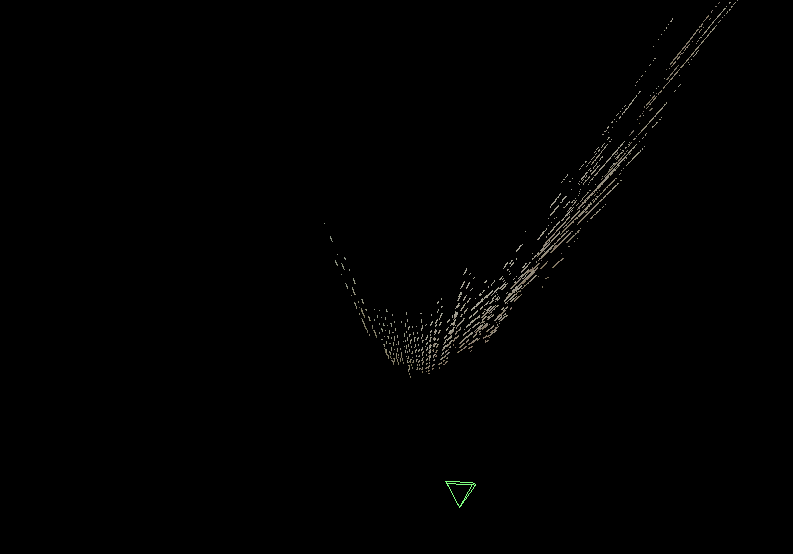
\includegraphics[width=0.85\linewidth]{includes/krumm.png}
		\caption{Scan einer geraden Wand bei falscher Kalibrierung}
		\label{fig:hw_calibration_fault}
	\end{figure}

\end{frame}

% ---------------------------------------------------------------------------- %

\section{Ergebnisse}

\begin{frame}
	\frametitlesec
	\framesubtitles{Messungen}
	
	\textbf{Messungen}
	
	\begin{figure}
		\begin{minipage}{0.32\linewidth}
			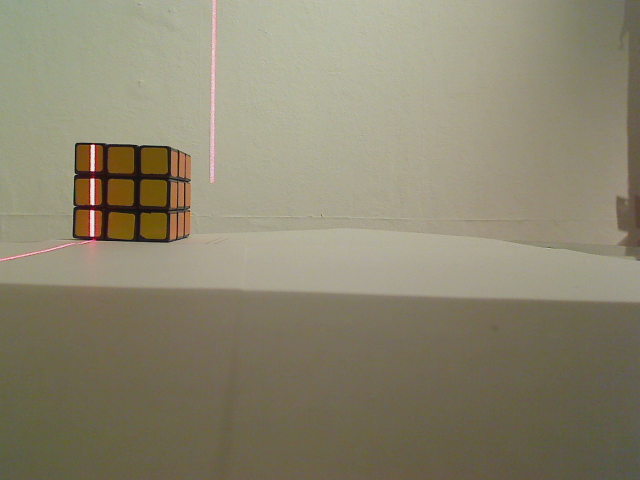
\includegraphics[width=\linewidth]{includes/test_repeat_1}
		\end{minipage}
		\hfill
		\begin{minipage}{0.32\linewidth}
			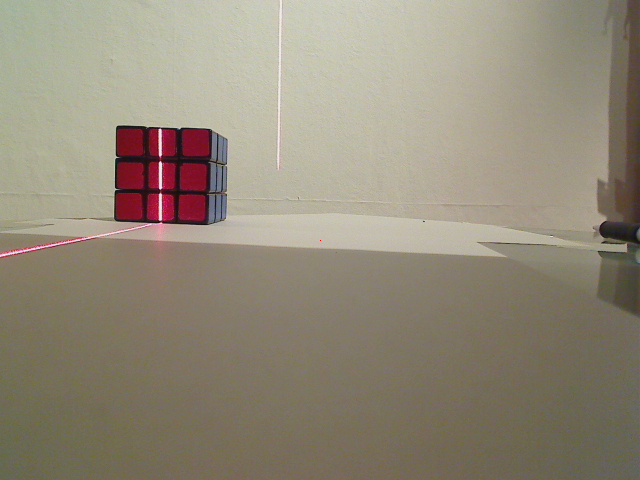
\includegraphics[width=\linewidth]{includes/test_repeat_2}
		\end{minipage}
		\hfill
		\begin{minipage}{0.32\linewidth}
			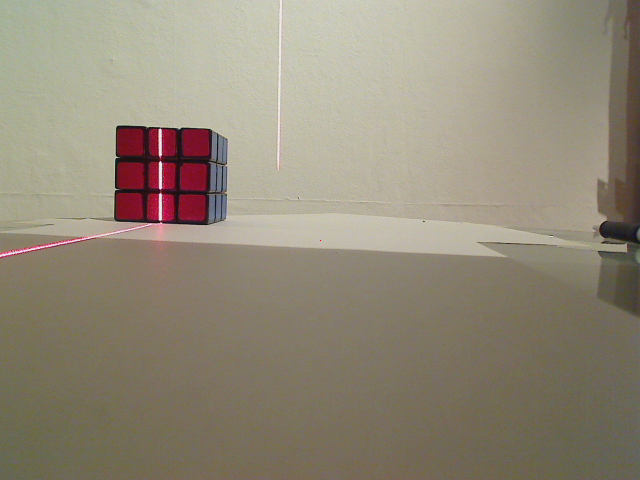
\includegraphics[width=\linewidth]{includes/test_repeat_3}
		\end{minipage}
	\end{figure}
	
	\begin{itemize}
		\item Pro Messung werden 71+1 Bilder aufgenommen
		\item Laser ist auf ca. 58 Bildern zu sehen
		\item Je Messung zwischen 10000 und 14000 (diff) \\ bzw. 21000 und 28000 (free) Punkte
		\item Davon gehören zwischen 750 und 1800 \\ bzw. 210 und 930 zum Würfel
	\end{itemize}


\end{frame}

%\subsection{Wiederholte Messungen}
\begin{frame}
	\frametitlesec
	\framesubtitles{Wiederholte Messungen}

	\textbf{Wiederholte Messungen}

	\begin{figure}
		\begin{minipage}{0.32\linewidth}
			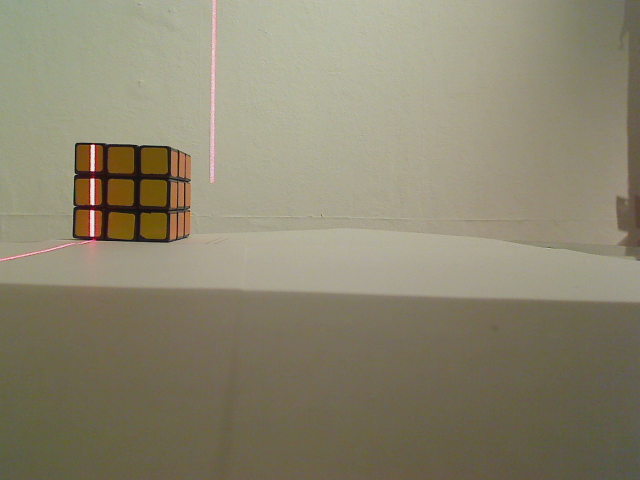
\includegraphics[width=\linewidth]{includes/test_repeat_1}
		\end{minipage}
		\hfill
		\begin{minipage}{0.32\linewidth}
			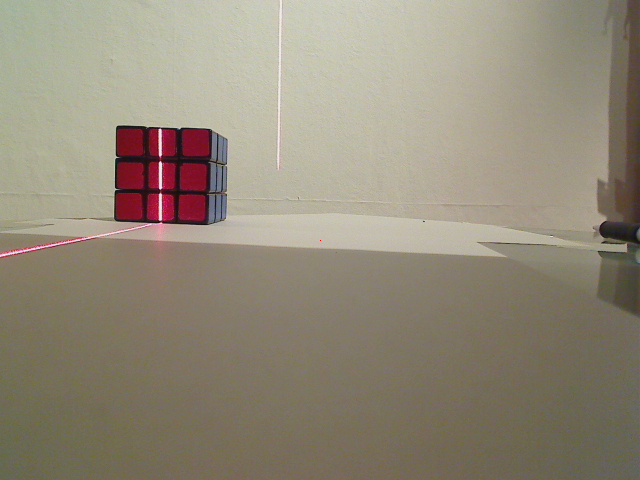
\includegraphics[width=\linewidth]{includes/test_repeat_2}
		\end{minipage}
		\hfill
		\begin{minipage}{0.32\linewidth}
			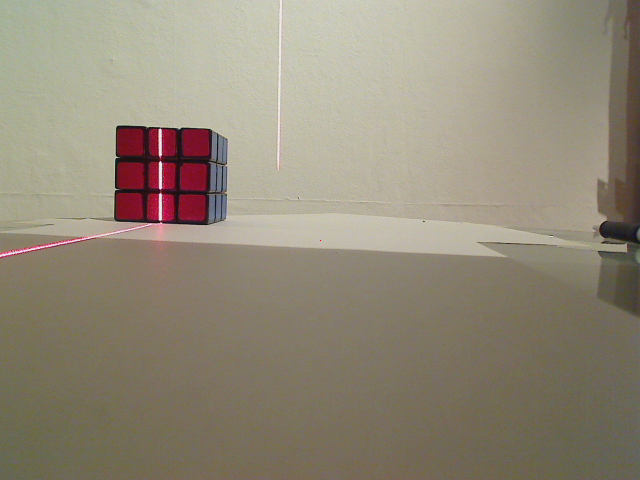
\includegraphics[width=\linewidth]{includes/test_repeat_3}
		\end{minipage}
	\end{figure}
	
	Entfernung: 300mm\\
	Höhe: 56mm\\
	Farbe: Gelb

\end{frame}
	
\begin{frame}
	\frametitlesec
	\framesubtitles{Wiederholte Messungen}
		\textbf{Entfernung}\\
	
		Linienerkennung mit Referenzbild\\
		Entfernung: 300mm
		
		\begin{tabular}{c|c|c|c|c|c}
			Messung & Min & Max & Avg & Diff (\%) & Stdabw \\ \hline
1 & 298.3 & 21629.5 & 348.7 & 16.2 & 909.1 \\
2 & 287.1 & 327.1 & 309.1 & 3.0 & 5.1 \\
3 & 287.1 & 327.1 & 309.9 & 3.3 & 6.0 \\
4 & 287.1 & 327.1 & 310.1 & 3.4 & 5.5 \\
5 & 287.1 & 458.0 & 310.2 & 3.4 & 7.3 \\
6 & 287.1 & 335.8 & 310.5 & 3.5 & 5.4 \\
7 & 299.8 & 15381.7 & 342.8 & 14.3 & 645.7 \\
8 & 299.0 & 327.1 & 309.4 & 3.1 & 5.0 \\
9 & 293.5 & 327.1 & 309.7 & 3.2 & 5.3 \\
10 & 287.1 & 11934.4 & 320.8 & 6.9 & 355.1
		\end{tabular}
		
\end{frame}
	
\begin{frame}
	\frametitlesec
	\framesubtitles{Wiederholte Messungen}
		\textbf{Entfernung}\\
	
		Linienerkennung ohne Referenzbild\\
		Entfernung: 300mm
		
		\begin{tabular}{c|c|c|c|c|c}
			Messung & Min & Max & Avg & Diff (\%) & Stdabw \\ \hline
1 & 300.7 & 325.1 & 307.6 & 2.5 & 4.3\\
2 & 77.0 & 323.1 & 243.1 & -19.0 & 101.2\\
3 & 300.7 & 325.1 & 307.9 & 2.6 & 4.3\\
4 & 77.0 & 327.1 & 250.7 & -16.4 & 97.4\\
5 & 300.7 & 327.1 & 307.9 & 2.6 & 4.1\\
6 & 77.0 & 327.1 & 246.4 & -17.9 & 99.7\\
7 & 300.7 & 323.1 & 307.5 & 2.5 & 3.8\\
8 & 300.7 & 327.1 & 308.1 & 2.7 & 4.3\\
9 & 77.0 & 323.1 & 251.1 & -16.3 & 97.3\\
10 & 80.2 & 325.1 & 278.0 & -7.3 & 75.6
		\end{tabular}
	
\end{frame}

\begin{frame}
	\frametitlesec
	\framesubtitles{Wiederholte Messungen}
		\textbf{Höhe}\\
		
		Höhe: 56mm
		
		\begin{tabular}{c|c}
		
		mit Referenzbild & ohne Referenzbild\\
		
		\begin{tabular}{c|c|c}
			Messung & Hoehe & Diff (\%) \\ \hline
1 & 48.6 & -13.2 \\
2 & 34.4 & -38.7 \\
3 & 27.8 & -50.3 \\
4 & 28.6 & -48.9 \\
5 & 49.2 & -12.2 \\
6 & 32.6 & -41.8 \\
7 & 27.2 & -51.3 \\
8 & 27.2 & -51.3 \\
9 & 34.4 & -38.7 \\
10 & 48.0 & -14.3\\

		\end{tabular} &
		
		
		\begin{tabular}{c|c}
			Hoehe & Diff (\%) \\ \hline
 54.8 &  -2.2 \\
 54.4 &  -2.9 \\
 54.7 &  -2.3 \\
 54.7 &  -2.3 \\
 54.7 &  -2.3 \\
 53.2 &  -4.9 \\
 53.9 &  -3.8 \\
 53.5 &  -4.4 \\
 53.5 &  -4.4 \\
 53.5 & -4.4 \\


		\end{tabular}
		
		\end{tabular}
\end{frame}


\begin{frame}
	\frametitlesec
	\framesubtitles{Verschiedene Farben}

	\textbf{Verschiedene Farben}

	\begin{figure}
		\begin{minipage}{0.32\linewidth}
			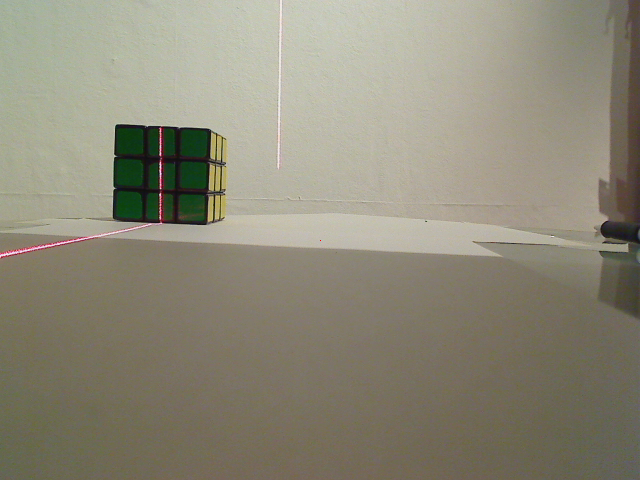
\includegraphics[width=\linewidth]{includes/test_color_1}
		\end{minipage}
		\hfill
		\begin{minipage}{0.32\linewidth}
			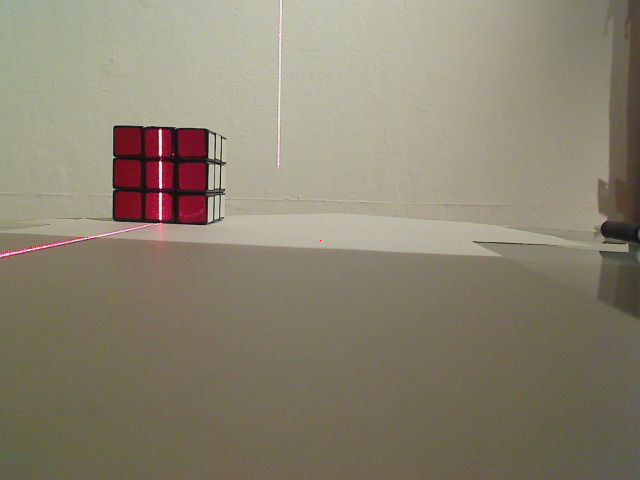
\includegraphics[width=\linewidth]{includes/test_color_2}
		\end{minipage}
		\hfill
		\begin{minipage}{0.32\linewidth}
			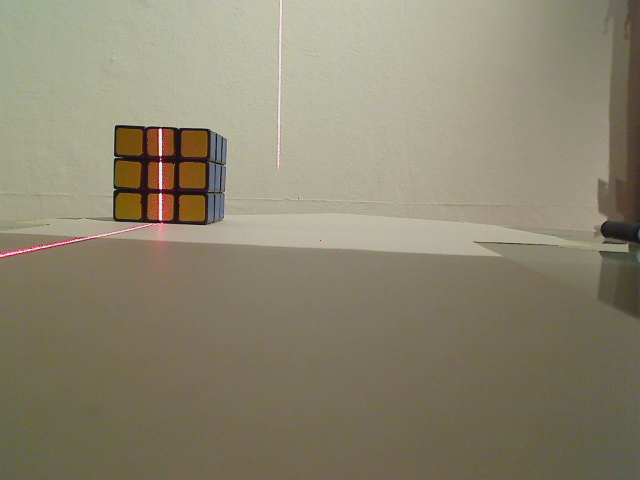
\includegraphics[width=\linewidth]{includes/test_color_3}
		\end{minipage}
	\end{figure}
	
	Entfernung: 300mm\\
	Höhe: 56mm\\
	je 10 Messungen
	
\end{frame}

\begin{frame}
	\frametitlesec
	\framesubtitles{Verschiedene Farben}
		\textbf{Entfernung}\\

		Entfernung: 300mm
		
		\begin{tabular}{c|c}		
		mit Referenzbild & ohne Referenzbild\\
		\begin{tabular}{c|c|c}
Farbe  & Avg & Stdabw\\ \hline
Blau   & 309.0 & 10.8\\
Grün   & 353.8 & 1054.2\\
Orange & 313.3 & 274.3\\
Rot    & 331.0 & 789.8\\
Gelb   & 318.3 & 379.5\\
		\end{tabular}
		
		& 
		
		\begin{tabular}{c|c}
Avg & Stdabw\\ \hline
310.7 & 18.3\\
301.2 & 47.8\\
309.8 & 186.2\\
306.2 & 21.6\\
276.5 & 77.8\\
		\end{tabular}
		
		\end{tabular}
\end{frame}

\begin{frame}
	\frametitlesec
	\framesubtitles{Verschiedene Farben}
		\textbf{Höhe}\\
		
		Höhe: 56mm
		
		\begin{tabular}{c|c}
		
		mit Referenzbild & ohne Referenzbild\\
		\begin{tabular}{c|c|c}
Farbe  & Avg  & Stdabw\\ \hline
Blau   & 55.5 & 0.8\\
Grün   & 58.1 & 14.2\\
Orange & 45.4 & 7.3\\
Rot    & 41.5 & 11.3\\
Gelb   & 35.8 & 8.8\\

		\end{tabular}
		&
		\begin{tabular}{c|c}
 Avg  & Stdabw\\ \hline
 55.1 & 1.0\\
 55.7 & 0.4\\
 55.4 & 0.3\\
 56.1 & 0.3\\
 54.8 & 0.6\\
		\end{tabular}
		
		\end{tabular}
		
\end{frame}


%\subsection{Verschiedene Entfernungen}
\begin{frame}
	\frametitlesec
	\framesubtitles{Verschiedene Entfernungen}
	
	\textbf{Verschiedene Entfernungen}

	\begin{figure}
		\begin{minipage}{0.32\linewidth}
			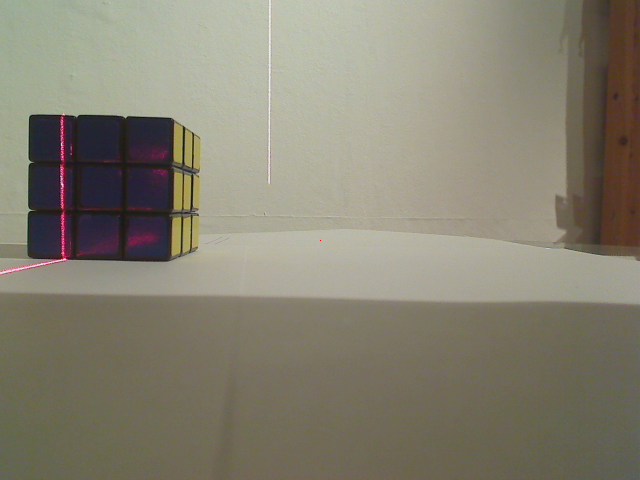
\includegraphics[width=\linewidth]{includes/test_dist_1}
		\end{minipage}
		\hfill
		\begin{minipage}{0.32\linewidth}
			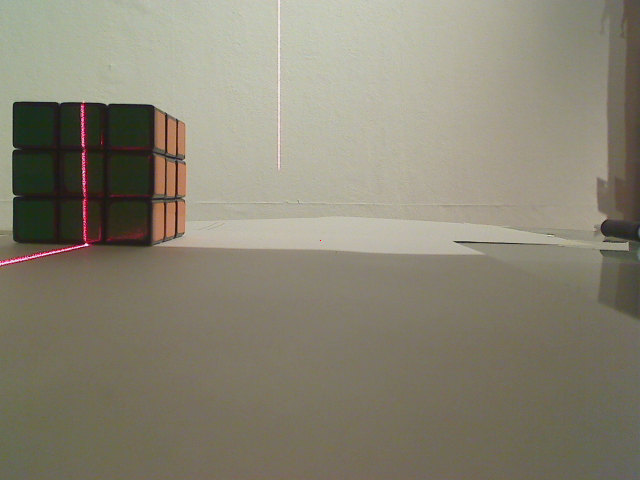
\includegraphics[width=\linewidth]{includes/test_dist_2}
		\end{minipage}
		\hfill
		\begin{minipage}{0.32\linewidth}
			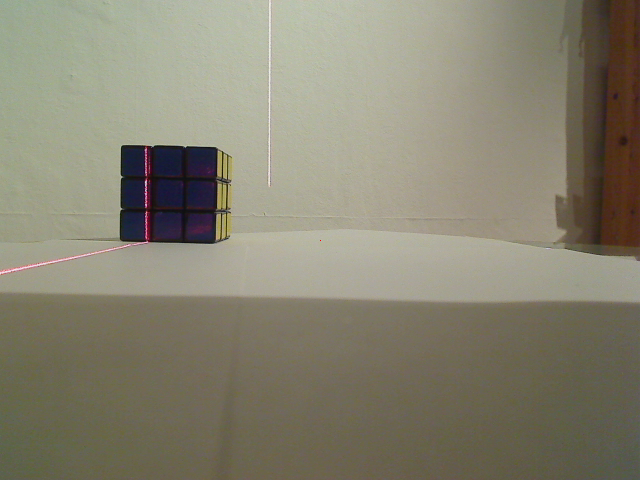
\includegraphics[width=\linewidth]{includes/test_dist_3}
		\end{minipage}
	\end{figure}
	Höhe: 56mm\\
	Farbe: Blau\\
	je 10 Messungen
	
\end{frame}

\begin{frame}
	\frametitlesec
	\framesubtitles{Verschiedene Entfernungen}
		\textbf{Entfernung}\\
		
		
		Entfernung: 300mm
		
		\begin{tabular}{c|c}
		
		mit Referenzbild & ohne Referenzbild\\
		
		\begin{tabular}{c|c|c}
Entfernung & Avg & Stdabw\\ \hline
150 &      172.6 & 34.7\\
200 &      215.4 & 23.3\\
250 &      261.8 & 15.6\\
300 &      309.0 & 10.8\\

		\end{tabular}
		&
		\begin{tabular}{c|c}
Avg   & Stdabw\\ \hline
146.6 & 48.3\\
210.9 & 31.5\\
261.0 & 21.9\\
310.7 & 18.3\\
		\end{tabular}
		
		\end{tabular}
		
		
\end{frame}

\begin{frame}
	\frametitlesec
	\framesubtitles{Verschiedene Entfernungen}
		\textbf{Höhe}\\
		
		Höhe: 56mm

		\begin{tabular}{c|c}
		
		mit Referenzbild & ohne Referenzbild\\		
		
		\begin{tabular}{c|c|c}
Entfernung & Avg & Stdabw\\ \hline
150 &      50.7 & 4.2\\
200 &      54.0 & 5.1\\
250 &      51.7 & 5.1\\
300 &      55.5 & 0.8\\

		\end{tabular}
		&
		
		\begin{tabular}{c|c}
Avg  &  Stdabw\\ \hline
36.0 &  12.6\\
55.8 &  0.5\\
54.9 & 0.4\\
53.8 & 1.0\\

		\end{tabular}
		\end{tabular}
\end{frame}



% ---------------------------------------------------------------------------- %

\section{Zusammenfassung und Ausblick}
\begin{frame}
	\frametitlesec
	
	\begin{columns}
	\column{.5\linewidth}{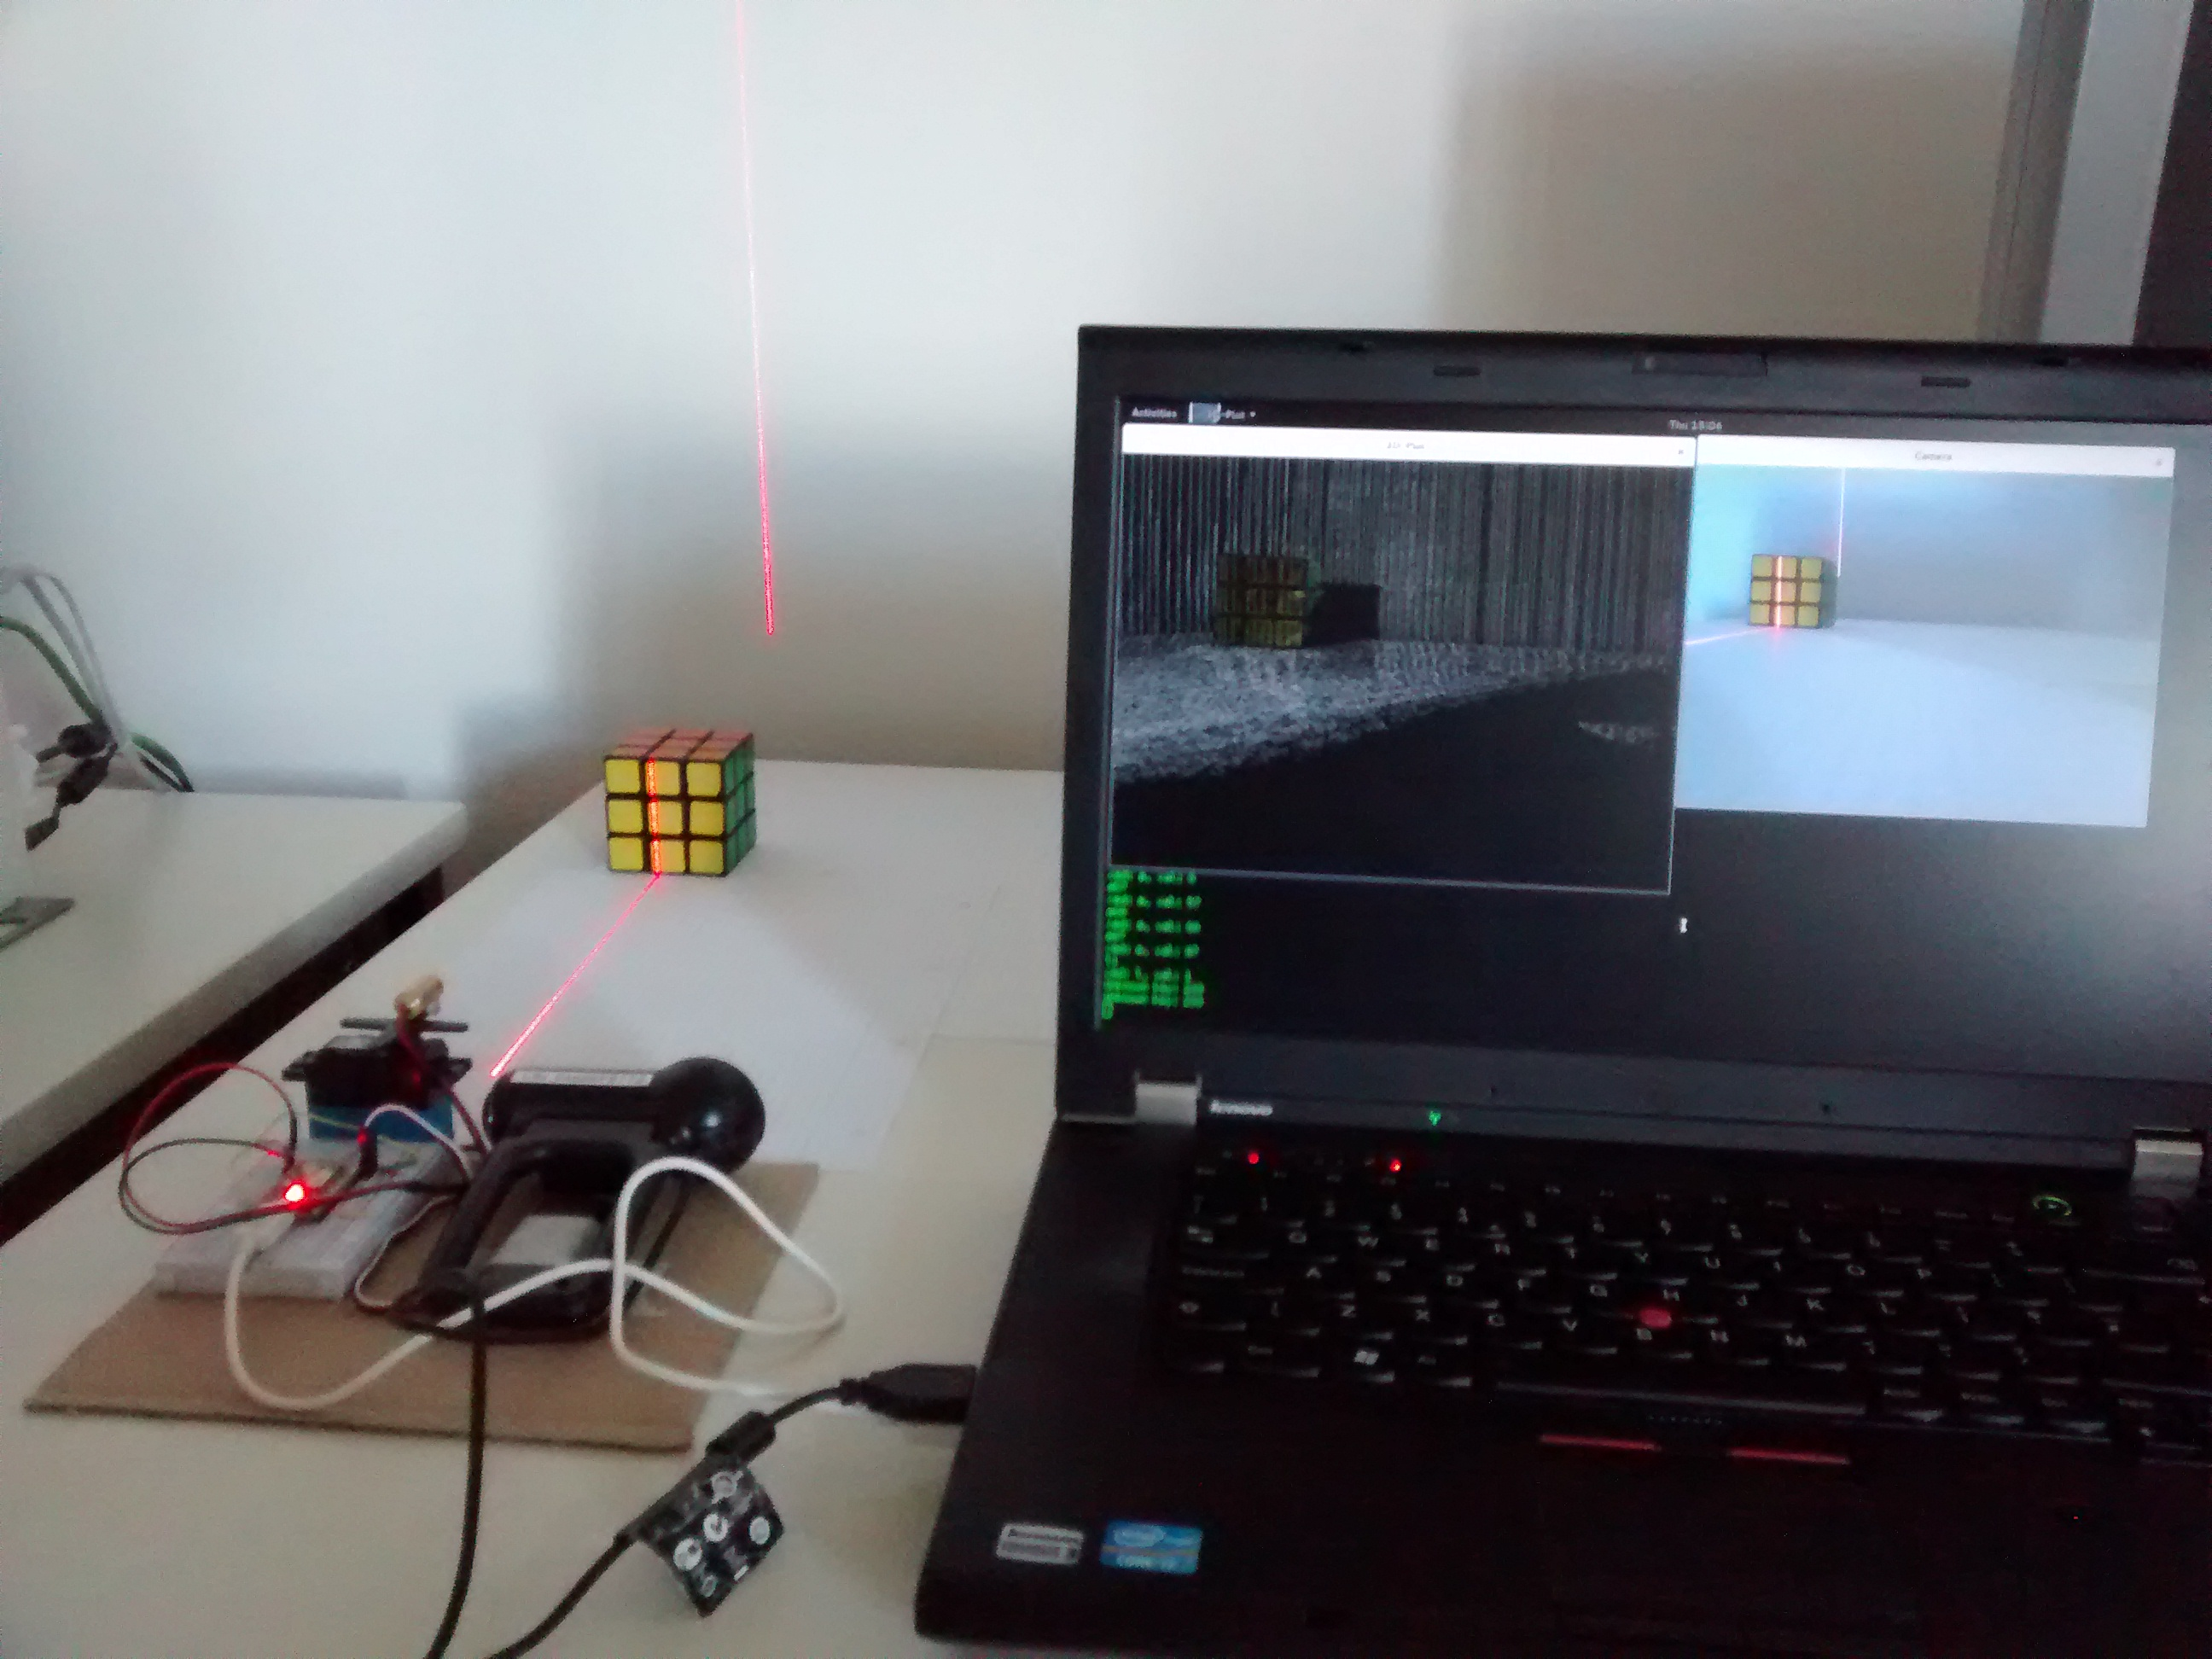
\includegraphics[width=\linewidth]{includes/setup}}
	\column{.5\linewidth}{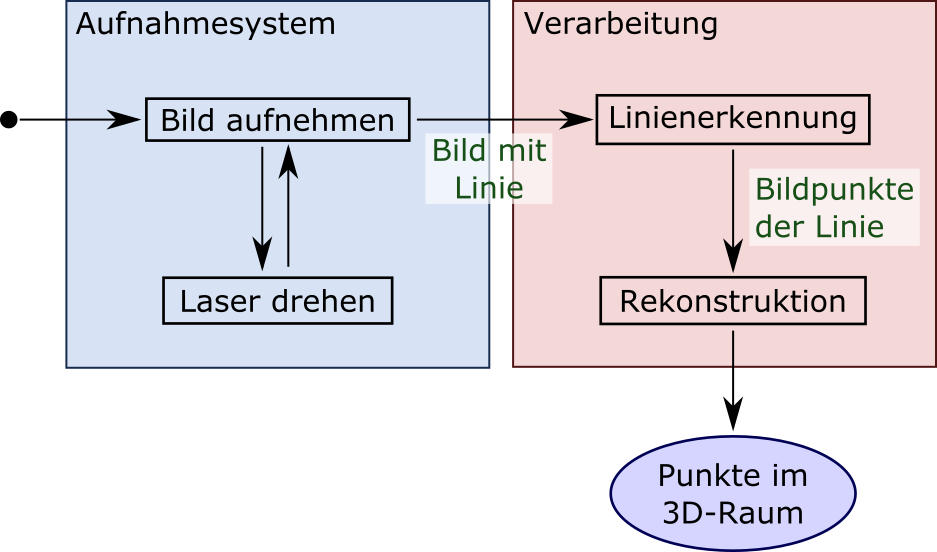
\includegraphics[width=\linewidth]{includes/blockbild.png}}
	\end{columns}
	\begin{columns}
	\column{.5\linewidth}{}
	\column{.4\linewidth}{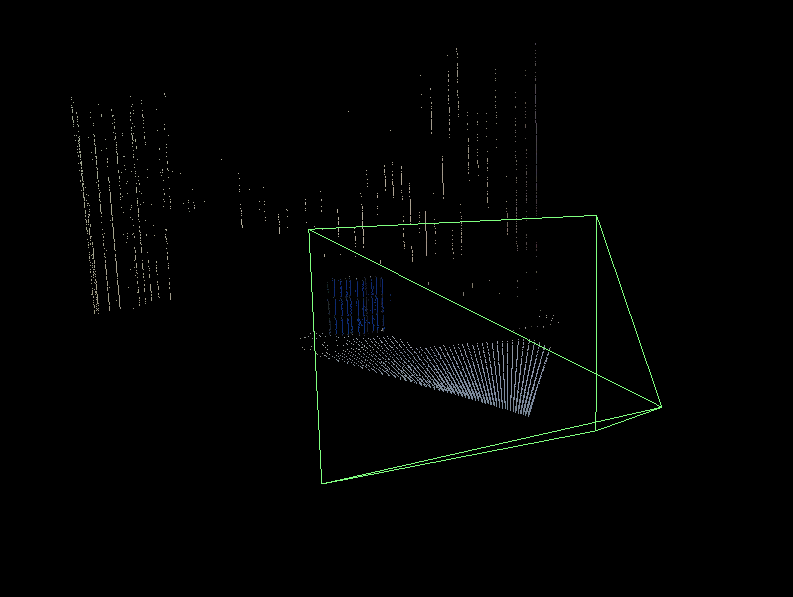
\includegraphics[width=\linewidth]{includes/3d_3.png}}
	\end{columns}

\end{frame}

\begin{frame}
	\frametitlesec
	
	\begin{itemize}
		\item Grobe Vermessung funktioniert
		\item Defizite bei der Genauigkeit durch ungenaue und/oder mangelhaft kalibrierte Hardware
	\end{itemize}
	
\end{frame}

\begin{frame}
	\frametitlesec

	\begin{itemize}
		\item Fehler durch bessere Kalibrierung und/oder besseres Setup minimieren
		\item Linienerkennung (ohne Referenzbild) robuster gestalten
		\item Objekt statt Laser bewegen
	\end{itemize}

\end{frame}

% ---------------------------------------------------------------------------- %

\begin{frame}
	\frametitle{Live-Demo}
\end{frame}

\begin{frame}
	\frametitle{\mbox{}}
	\center \LARGE Vielen Dank für eure Aufmerksamkeit!
\end{frame}



%\subsection{Verschiedene Farben}
\section*{Anhang}
\begin{frame}
	\frametitlesec
	\framesubtitles{Verschiedene Farben}

	\textbf{Verschiedene Farben}

	\begin{figure}
		\begin{minipage}{0.32\linewidth}
			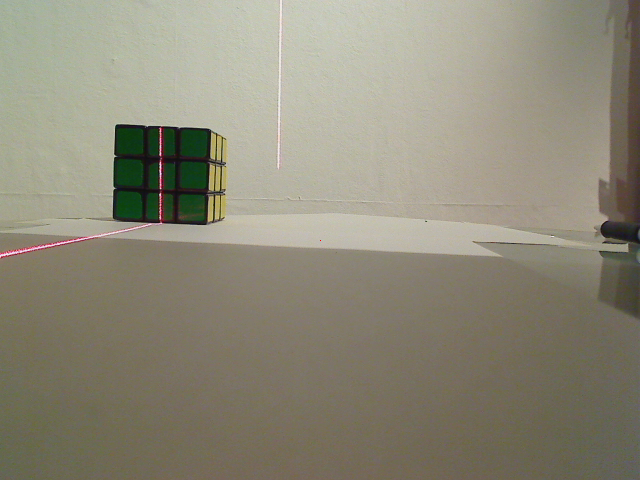
\includegraphics[width=\linewidth]{includes/test_color_1}
		\end{minipage}
		\hfill
		\begin{minipage}{0.32\linewidth}
			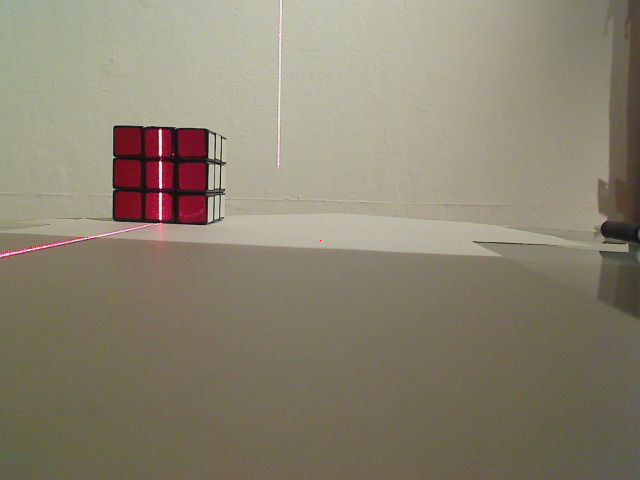
\includegraphics[width=\linewidth]{includes/test_color_2}
		\end{minipage}
		\hfill
		\begin{minipage}{0.32\linewidth}
			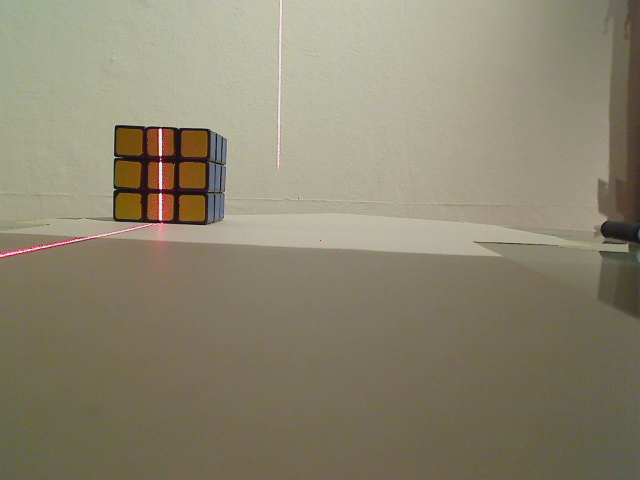
\includegraphics[width=\linewidth]{includes/test_color_3}
		\end{minipage}
	\end{figure}
	
	Entfernung: 300mm\\
	Höhe: 56mm\\
	je 10 Messungen
	
\end{frame}
	
\begin{frame}
	\frametitlesec
	\framesubtitles{Verschiedene Farben}
		\textbf{Entfernung}\\
		
		Linienerkennung mit Referenzbild\\
		Entfernung: 300mm
		\begin{tabular}{c|c|c|c|c|c}
			Farbe & Min & Max & Avg & Diff (\%) & Stdabw\\ \hline
Blau &-1.3 & 351.5 & 309.0 & 3.0 & 10.8\\
Grün &-1.3 & 36424.6 & 353.8 & 17.9 & 1054.2\\
Orange &-1.3 & 21629.5 & 313.3 & 4.4 & 274.3\\
Rot &-1.3 & 36424.6 & 331.0 & 10.3 & 789.8\\
Gelb &-1.3 & 21629.5 & 318.3 & 6.1 & 379.5\\
		\end{tabular}
		
\end{frame}

\begin{frame}
	\frametitlesec
	\framesubtitles{Verschiedene Farben}
		\textbf{Entfernung}\\
		
		Linienerkennung ohne Referenzbild\\
		Entfernung: 300mm
		
		\begin{tabular}{c|c|c|c|c|c}
			Farbe & Min & Max & Avg & Diff (\%) & Stdabw\\ \hline
Blau &-1.3 & 325.1 & 310.7 & 3.6 & 18.3\\
Grün &-1.3 & 325.1 & 301.2 & 0.4 & 47.8\\
Orange &-1.3 & 15381.7 & 309.8 & 3.3 & 186.2\\
Rot &-1.3 & 329.1 & 306.2 & 2.1 & 21.6\\
Gelb & -1.3 & 327.1 & 276.5 & -7.8 & 77.8\\
		\end{tabular}

\end{frame}


\begin{frame}
	\frametitlesec
	\framesubtitles{Verschiedene Farben}
		\textbf{Höhe}\\
		
		Linienerkennung mit Referenzbild\\
		Höhe: 56mm
		
		\begin{tabular}{c|c|c|c|c|c}
			Farbe & Min & Max & Avg & Diff (\%) & Stdabw\\ \hline
Blau &   54.3 & 56.4 & 55.5 & -0.8 & 0.8\\
Grün &    39.9 & 98.4 & 58.1 & 3.8 & 14.2\\
Orange&     32.0 & 56.1 & 45.4 & -19.0 & 7.3\\
Rot &    29.8 & 69.9 & 41.5 & -25.9 & 11.3\\
Gelb &     27.2 & 49.2 & 35.8 & -36.1 & 8.8\\

		\end{tabular}
		
		
\end{frame}

\begin{frame}
	\frametitlesec
	\framesubtitles{Verschiedene Farben}
		\textbf{Höhe}\\
		
		Linienerkennung ohne Referenzbild\\
		Höhe: 56mm
		
		\begin{tabular}{c|c|c|c|c|c}
			Farbe & Min & Max & Avg & Diff (\%) & Stdabw\\ \hline
Blau &    52.1 & 55.1 & 53.8 & -3.9 & 1.0\\
Grün &     54.2 & 55.7 & 54.9 & -2.0 & 0.4\\
Orange&     54.5 & 55.4 & 54.6 & -2.4 & 0.3\\
Rot &    54.7 & 56.1 & 55.2 & -1.4 & 0.3\\
Gelb &      53.2 & 54.8 & 54.1 & -3.4 & 0.6\\

		\end{tabular}
		
		
\end{frame}


%\subsection{Verschiedene Entfernungen}
\begin{frame}
	\frametitlesec
	\framesubtitles{Verschiedene Entfernungen}
	
	\textbf{Verschiedene Entfernungen}

	\begin{figure}
		\begin{minipage}{0.32\linewidth}
			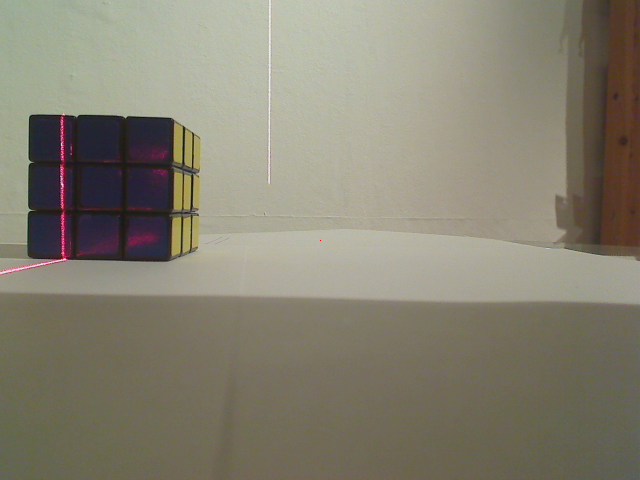
\includegraphics[width=\linewidth]{includes/test_dist_1}
		\end{minipage}
		\hfill
		\begin{minipage}{0.32\linewidth}
			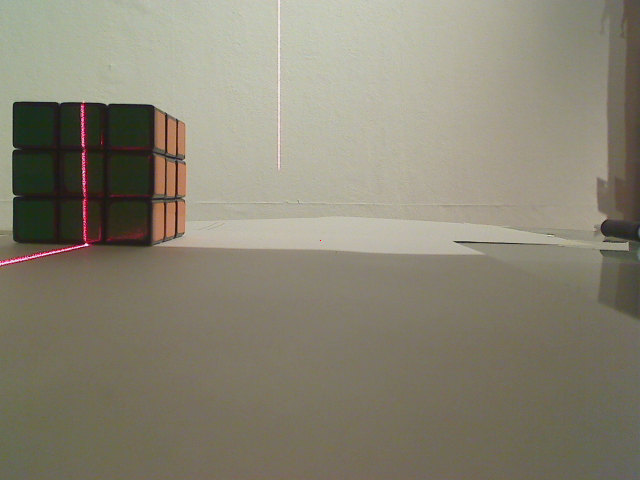
\includegraphics[width=\linewidth]{includes/test_dist_2}
		\end{minipage}
		\hfill
		\begin{minipage}{0.32\linewidth}
			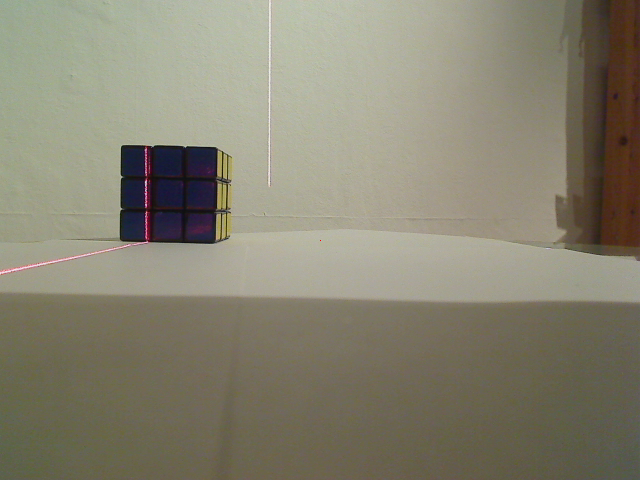
\includegraphics[width=\linewidth]{includes/test_dist_3}
		\end{minipage}
	\end{figure}
	Höhe: 56mm\\
	Farbe: Blau\\
	je 10 Messungen
	
\end{frame}

\begin{frame}
	\frametitlesec
	\framesubtitles{Verschiedene Entfernungen}
		\textbf{Entfernung}\\
		
		Linienerkennung mit Referenzbild\\
		Entfernung: 300mm
		
		\begin{tabular}{c|c|c|c|c|c}
			Entfernung & Min & Max & Avg & Diff (\%) & Stdabw\\ \hline
150 &      -1.3 & 477.4 & 172.6 & -42.5 & 34.7\\
200 &      -1.3 & 392.0 & 215.4 & -28.2 & 23.3\\
250 &      -1.3 & 864.4 & 261.8 & -12.7 & 15.6\\
300 &      -1.3 & 351.5 & 309.0 & 3.0 & 10.8\\

		\end{tabular}
		
		
\end{frame}

\begin{frame}
	\frametitlesec
	\framesubtitles{Verschiedene Entfernungen}
		\textbf{Entfernung}\\
		
		Linienerkennung ohne Referenzbild\\
		Entfernung: 300mm
		
		\begin{tabular}{c|c|c|c|c|c}
			Entfernung & Min & Max & Avg & Diff (\%) & Stdabw\\ \hline
150 &      -1.3 & 398.8 & 146.6 & -51.1 & 48.3\\
200 &      -1.3 & 375.2 & 210.9 & -29.7 & 31.5\\
250 &      -1.3 & 375.2 & 261.0 & -13.0 & 21.9\\
300 &   -1.3 & 325.1 & 310.7 & 3.6 & 18.3\\
		\end{tabular}

\end{frame}



\begin{frame}
	\frametitlesec
	\framesubtitles{Verschiedene Entfernungen}
		\textbf{Höhe}\\
		
		Linienerkennung mit Referenzbild\\
		Höhe: 56mm
		
		\begin{tabular}{c|c|c|c|c|c}
			Entfernung & Min & Max & Avg & Diff (\%) & Stdabw\\ \hline
150 &     39.1 & 56.6 & 50.7 & -9.5 & 4.2\\
200 &     42.4 & 57.3 & 54.0 & -3.6 & 5.1\\
250 &     43.6 & 56.8 & 51.7 & -7.6 & 5.1\\
300 &  54.3 & 56.4 & 55.5 & -0.8 & 0.8\\


		\end{tabular}
\end{frame}


\begin{frame}
	\frametitlesec
	\framesubtitles{Verschiedene Entfernungen}
		\textbf{Höhe}\\
		
		Linienerkennung ohne Referenzbild\\
		Höhe: 56mm
		
		\begin{tabular}{c|c|c|c|c|c}
			Entfernung & Min & Max & Avg & Diff (\%) & Stdabw\\ \hline
150 &     21.9 & 56.7 & 36.0 & -35.6 & 12.6\\
200 &     54.9 & 56.5 & 55.8 & -0.4 & 0.5\\
250 &     54.4 & 55.9 & 54.9 & -1.9 & 0.4\\
300 &     52.1 & 55.1 & 53.8 & -3.9 & 1.0\\

		\end{tabular}
\end{frame}

\end{document}
